% TODO: Ableitungen und Schaubilder einfügen
\section{Activation Functions}
\label{sect:activation-functions}
The activation functions should have the following properties:
\begin{itemize}
	\item continous
	\item bounded
	\item monotonically increasing
	\item differentiable
\end{itemize}
\subsection{Step Function}
\label{ssect:linear-function}
\[
\varphi(x) = \begin{cases}
1 \: \text{if} x > 0 \\
0 \: \text{if} x \leq 0 \\
\end{cases}
\]
Derivative is always 0
\subsection{Linear Function}
\label{ssect:linear-function}
\[
\varphi(x) = x
\]
Linear functins alone can only solve linear separable problems but can be used in a combination node for function approximation problems.
\subsection{Logistic / Sigmoid Function}
\label{ssect:logistic-function}
\begin{align*}
\varphi(x) = sigmoid(x) &= \frac{1}{1 + e^{-x}} \\
\frac{\delta \varphi(x)}{\varphi(x)} &= \varphi(x) (1 - \varphi(x))
\end{align*}
Good for internal nodes, bad for outpur nodes.
\begin{figure}[h]
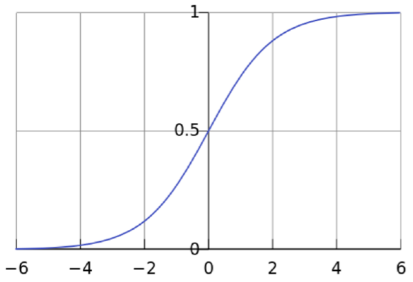
\includegraphics[scale=0.4]{sigmoid}
\end{figure}

\subsection{Hyperbolic Tangent function}
\label{ssect:hyperbolic-tangent-function}
\begin{align*}
\sigma(x) = \tanh(x) &= \frac{e^x - e^{-x}}{e^x + e^{-x}} \\
\frac{\delta \sigma(x)}{\sigma(x)} = 1 - \tanh^2(x) &= 1 - \frac{(e^x - e^{-x})^2}{(e^x + e^{-x})^2}
\end{align*}
\begin{figure}[h]
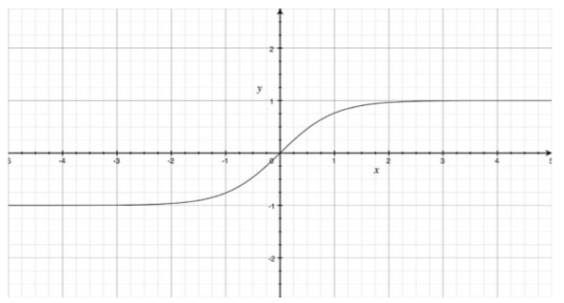
\includegraphics[scale=0.6]{tanh}
\end{figure}
If the input has a mean of 0 then so will the output

\subsection{Softmax Function}
\label{ssect:softmax-function}
\begin{align*}
\varphi(x_j) &= \frac{e^{x_j}}{\sum_k e^{x_k}} \\
\frac{\delta \varphi(x_j)}{\varphi(x_j)} = \varphi(x_j) - \varphi(x_j)^2 &= \varphi(x_j)(1 - \varphi(x_j))
\end{align*}
Outputs an a posteriori probability $p(c | x)$ and is good for classification tasks.

\subsection{Rectified Linear Unit}
\label{ssect:softmax-function}
\begin{align*}
s
\end{align*}
\newpage